\textbf{\Large Аннотация}

В работе изучаются свойства полупроницаемых перегородок. Измеряется осмотическое давления при разной концентрации кровяной соли. 

\textbf{\Large Теория}

\textit{Полупроницаемой перегородкой} называется перегородка, которая пропускает молекулы растворителя, но не пропускает молекулы растворённых в ней соединений. Прохождение растворителя через полупроницаемую перегородку называется \textit{осмосом}.

\begin{wrapfigure}{r}{0.42\textwidth}
	\centering
	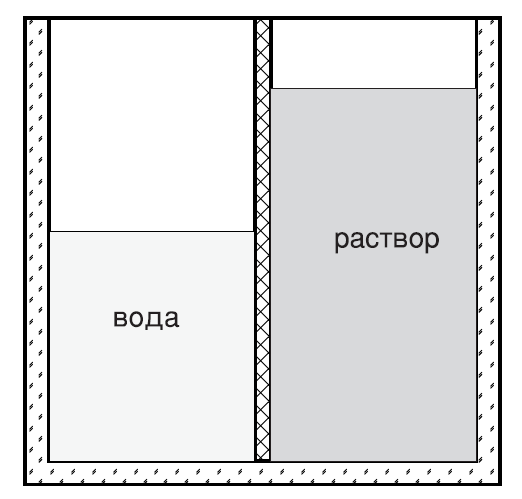
\includegraphics[width=0.4\textwidth]{../images/scheme_theory.png}
\end{wrapfigure}

Рассмотрим сосуд, разделённый на две части полупроницаемой перегородкой. По одну сторону находится вода, по другую ~---~ водный раствор вещества, молекулы которого не могут проходить через перегородку. Наполним обе части сосуда до одинакового уровня. Опыт показывает, что вода начинает переходить в ту часть сосуда, где содержится раствор. Этот переход продолжается до тех пор, пока между водой и раствором не установится некоторая разность уровней, а следовательно, и разность давлений, которая называется \textit{осмотическим давлением}.

Опыт показывает, что осмотическое давление для весьма разбавленных растворов численно равно давлению, которое оказывало растворенное вещество, если бы оно при данной температуре находилось в состоянии идеального газа и занимало бы объём, равный объёму сосуда. Данное соотношение называется законом Вант-Гоффа:
$$
P_{осм} = n k T
$$ \\
где $n$ ~---~ концентрация растворенного вещества, $k_Б$ ~---~ постоянная Больцмана, $T$ ~---~ температура.

\newpage

\textbf{\Large Методика измерения}

Приборы, служащие для измерения осмотического давления, называются \textit{осмометрами}. Прохождение растворителя через полупроницаемую перегородку происходит медленно, так что равновесие устанавливается не скоро. Для ускорения измерений, над раствором создают избыточное давление воздуха. Если избыточное давление равно осмотическому, то переход растворителя через перегородку прекращается. Если же оно превышает осмотическое давление, то растворитель переходит через перегородку в обратном направлении. Таким образом измерение осмотического давления сводится к измерению равновесного давления газа.

Для определения $P_{осм}$ измеряется изменение скорости $v$ движения уровня раствора в капилляре в зависимости от давления $P$ и строится график зависимости $v(P)$. Чем больше разность давлений $P - P_{осм}$, тем больше скорость $v$ движения уровня в капилляре. При $P \approx P_{осм}$ эта скорость равна 0. Поэтому измерения следует проводить либо при $P \gg P_{осм}$, либо при $P \ll P_{осм}$. По графику определяется значение $P$, при котором $v = 0$, то есть осмотическое давление.
